\chapter{Введение} % черновой вариант текста [изменения неизбежны]
% Что почитать
% http://habrahabr.ru/post/250745/
% http://habrahabr.ru/company/mosigra/blog/177249/
% http://inwebwetrust.org/trust/Game_Development_Dynamics_Playdeck.html
% https://developer.valvesoftware.com/wiki/Game_Mechanics_%28Portal_2%29:ru

% http://habrahabr.ru/post/255561/

В данном методическом руководстве я не буду давать информацию по установке и настройке компиляторов и 
сред разработки, так же как и советовать использовать конкретный язык программирования. Я попытаюсь 
изложить некоторые тонкости в разработке структуры игровых программ: частые ошибки, возможные проблемы и 
на что стоит обратить внимание при проектировании и разработке.

Примеры в основном будут на языке C++ с использованием следующих библиотек:
\begin{itemize}
    \item SDL2
    \item OpenGL
    \item GLUT
    \item OpenAL
    \item vorbis
\end{itemize}

Я глубоко надеюсь что прежде чем разрабатывать игру читатель определил для себя: \emph{идею}, \emph{жанр}, 
\emph{история}, \emph{стиль}, \emph{игровая механика} разрабатываемой игры. Но не стоит расстраиваться если 
у вас нет ещё идеи для игры -- давайте вместе шаг за шагом рассмотрим и напишем ремейк старой игры под 
названием Asteroids.

\chapter{Основа игровой программы}
\section{Введение}
С чего начинается проектирование игры? Обычно всё начинается с идеи. Наверное самый важный компонент 
любой игры. Конечно она может быть не столь яркой и интересной, но определив игровую механику можно 
сгладить этот изъян и получить довольно интересную и яркую игру. Немаловажным является то, что если у 
разрабатываемой игры появляется своя история и неповторимый стиль, которые только развивают идею и 
улучшают возникаемые впечатления от игры.

Но не будем филосовствовать на этот счёт и подойдём с другой стороны -- с технической. Для того чтобы начать
разрабатывать игру с нуля нам нужен некоторый \emph{скелет} (в другом случае -- использовать функции 
используемого фреймворка).

\section{Проектирование структуры игры}

Если говорить в общем, то самую простую структуру можно представить блок схемой \ref{img:skeleton}.
% картинка с 
% Инициализация -> Обработка событий -> Игровой цикл -> Рендеринг +-> Деинициализация
%                  ^-----------------------------------------------
\begin{wrapfigure}[18]{r}{0.22\linewidth}
    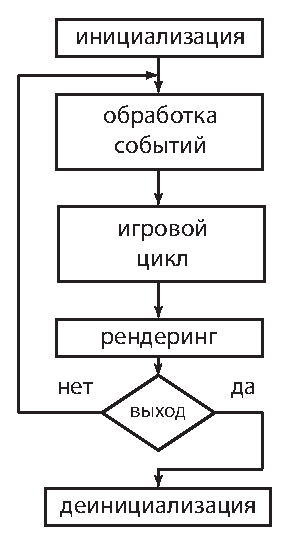
\includegraphics[width=0.2\textwidth]{game_loop}
    \caption{Структура игрового цикла}
    \label{img:skeleton}
\end{wrapfigure}

На этом простом \emph{скелет} мы и разработаем игровую программы. Конечно используемые \emph{скелеты} в 
профессиональной сфере могут (и будут) иметь более сложную структура, но для разработки простых игр, нам 
хватит и данной структуры.

Давайте рассмотрим каждый шаг в этой схеме. \textbf{Инициализация} -- блок подготовки и предобработки 
игровыхданных. Это может быть пред-/загрузка графических, звуковых и конфигурационных файлов. Список может 
быть и больше, в зависимости от конкретного типа игры: игровые карты, получение информации с игрового 
сервера, генерация параметров игровых предметов и многое другое. Говоря в общем -- это подготовка данных 
для игры.

Блок \textbf{обработки событий} в основном отвечает за работу с оконной системой, т.е. нажатая клавиша, 
передвинутый курсор, изменение размера окна программы и прочие события связанные с окном программы в 
операционной системе. 

Далее у нас по списку -- \textbf{игровой цикл}. Проводя аналогию с предыдущим блоком, то этот блок делает 
тоже самое, но для нашей игры -- двигает персонажей, обрабатывает игровые события и многие другие вещи, 
которые нам нужны в играх. Этот блок можно конечно разделить на много мелких, которые отвечают за 
отдельные части игровой программы, но мы остановимся на более общем виде. 

Ну и последнее в цикле это \textbf{рендеринг} -- основная часть структуры программы, без которой мы не могли 
бы представить пользователю графическую часть нашей игры. Всё что связано с обработкой и отрисовкой графики 
располагается здесь: от шейдеров до рисования точки на экране.

Внимательный читатель мог заметить и сказать: -- А где собственно работа со звуком? И он будет прав, в нашей 
структуре отсутствует звуковая система! Если быть честным, то звуковая система должна быть идти сразу после 
инициализации, но для того чтобы мы не слышали обрывки в воспроизведении звука она должна идти отдельным 
потоком. Таким образом звуковая система будет работать параллельно нашему циклу и не зависеть от его скорости 
выполнения. Также можно сказать, что стоит выносить в отдельный поток и рендеринг, так как при во многих 
случаях нужно обеспечивать приемлемую скорость его работы, а в данном потоке это не является возможным. 
Но так как наша игра не будет столь требовательной к скорости работы, то мы можем оставить всё как есть.

И наконец последний блок \textbf{деинициализация} -- освобождение выделенных в первом блоке ресурсов и 
устройств. Важный блок с точки зрения работы с памятью.

\section{Программная реализация скелета}
Давайте напишем \emph{скелет} программы шаг за шагом на примере работы с двумя разными библиотеками 
SDL2 и GLUT.

Для начала нам нужно выделить основные блоки, которые будут одинаковы в каждой программе независимо от 
используемой библиотеки, а также не забываем о предыдущем пункте, где мы рассматривали структуру типичной 
игровой программы.

\begin{lstlisting}
    void game_init( void ) { // инициализация }
    void game_event( void ) { // обработка событий }
    void game_loop( void ) { // игровой цикл }
    void game_render( void ) { // функция рендеринга }
    void game_destroy( void ) { // деинициализация }
    int main( int argc, char * argv[] ) {
        // точка входа в программу
        return EXIT_SUCCESS;
    }
\end{lstlisting}

Данный код больше подходить к использованию с библиотекой SDL2, в тоже время библиотека GLUT требует 
объявления \emph{callback}-функций, которые будут обрабатывать определенные события. Как пример приведу 
изменения, которые нужно совершить, чтобы удовлетворить программную архитектуру библиотеки GLUT.
\begin{lstlisting}
    void game_init( void ) { // инициализация }
    void game_...( <params> ) { // callback функции }
    void game_loop( int value ) { // игровой цикл }
    void game_render( void ) { // функция рендеринга }
    void game_destroy( void ) { // деинициализация }
    int main( int argc, char * argv[] ) {
        // точка входа в программу
        return EXIT_SUCCESS;
    }
\end{lstlisting}

Троеточием показано, что название функции будет зависеть от того, что мы хотим использовать: обработку 
событий от клавиатуры, мыши, окна и прочие. Давайте в текущем примере используем обработчик клавиатуры, но 
для этого определим параметры, которые нам будут нужны для работы с окном.

SDL2:
\lstinputlisting[firstline=3, lastline=13]{../game/01_init/src/sdl2_init.cpp}

GLUT:
\lstinputlisting[firstline=3, lastline=10]{../game/01_init/src/glut_init.cpp}

Основные параметры на которые стоит обратить внимание: \textbf{name} -- имя окна, \textbf{width} -- ширина, 
\textbf{height} -- высота. Это постоянные параметры, которые не будут меняться, а остальные зависят от 
используемой библиотеки. В случае с SDL2: \textbf{window} -- идентификатор окна, \textbf{render} -- контекст 
отрисовщика, \textbf{event} -- структура хранящая оконные события. Для GLUT пока только одно специфическое 
\textbf{win\_id} -- идентификатор окна.

Теперь можно перейти к определению функции обработки событий клавиатуры.

GLUT:
\lstinputlisting[firstline=25, lastline=38]{../game/01_init/src/glut_init.cpp}

В данном отрывке кода представлено два события: закрытие окна по нажатию на клавишу 'q' и переключение между 
режимами экрана 'f'.

Основные функции:
\begin{itemize}
    \item glutDestroyWindow( GLint window\_handle ) -- уничтожение окна по идентификатору
    \item glutFullScreen( GLvoid ) -- переход в полноэкранный режим
    \item glutReshapeWindow( GLint width, GLint height ) -- изменение размера окна
\end{itemize}

Далее рассмотрим использование каждой библиотеки по отдельности.

\subsection{SDL2}
Давайте постепенно функция за функцией опишем \textbf{скелет} программы. Первое с чего начнём -- функция 
обработки ошибок. В дальнейшем она нам будет очень полезна, да и пользователь сможет понять что случилось при 
экстренном закрытии программы.

\lstinputlisting[firstline=15, lastline=20]{../game/01_init/src/sdl2_init.cpp}

Библиотечная функция \emph{SDL\_ShowSimpleMessageBox} принимает несколько параметров на вход, а именно:
\begin{enumerate}
    \item тип икона
    \item заголовок окна
    \item выводимое сообщение
    \item тип используемых кнопок (если ноль или \textbf{nullptr}, то кнопка OK)
\end{enumerate}

Код прозрачен и прост -- в случае ошибки мы выводим её на экран, а далее закрываем программы с 
соответствующим кодом. 

Идём далее и реализуем код для точки входа в программу используя рис.~\ref{img:skeleton}.
\lstinputlisting[firstline=87, lastline=97]{../game/01_init/src/sdl2_init.cpp}

Главное на что стоит обратить внимание, так это параметр \textbf{quit\_flag}, который будет сигнализировать 
нам о закрытии программы. В остальном всё соответствует рис.~\ref{img:skeleton}.

Теперь пойдём последовательно по блокам и опишем каждый из них. Начнём с рассмотрения псевдокода, а потом 
рассмотрим на примере работающего кода.

Всё что нужно, чтобы инициализировать систему на данном этапе, так это несколько шагов:
\begin{enumerate}
    \item инициализировать SDL2
    \item создать окно
    \item создать контекст отрисовщика
    \item обработать предыдущие шаги на ошибки
\end{enumerate}

Так давайте сделаем это:

\lstinputlisting[firstline=68, lastline=85]{../game/01_init/src/sdl2_init.cpp}

Рассмотрим кратко каждую из них (так как подробно описано в вики проекта \cite{sdl2wiki}).

\begin{itemize}
    \item SDL\_Init -- инициализация систем SDL2 (видео, аудио, клавиатура \ldots)
    \item SDL\_CreateWindow -- создание окна приложения
    \item SDL\_CreateRender -- функция инициализации контекста отрисовщика
\end{itemize}

Блоки, где производятся сравнения с нулевым указателем -- это обработка ошибок.

Далее следует блок обработки событий. На этапе проектирования он будет иметь минимальный функционал:
\begin{itemize}
    \item обработка закрытия программы
    \item обработка изменения размера окна
    \item шаблон для обработки нажатия клавиш
\end{itemize}

В программном коде это будет выглядеть так:
\lstinputlisting[firstline=22, lastline=47]{../game/01_init/src/sdl2_init.cpp}

При вызове данной функции происходит следующее: с помощью \emph{SDL\_PollEvent} мы запрашиваем текущее 
событие от системы SDL2, а далее с помощью конструкции \textbf{switch-case} выбираем соответствующую 
ветку для обработки. Всего их сейчас три, не считая \textbf{default}. 

Первая \emph{SQL\_QUIT} -- отвечает за обработку события выхода из программы -- в нашем случае это 
установка булевой функции в значение \textbf{true}, что обеспечит нам выход из основного цикла.

Вторая \emph{SDL\_WINDOWEVENT} и последующее за ним условие \emph{SDL\_WINDOWEVENT\_RESIZED} отвечают 
за изменение размеров окна и соответствующее внесение изменения в параметры нашей структуры 
(\emph{gw.width} и \emph{gw.height}).

И последнее событие \emph{SDL\_KEYDOWN} отвечающее за нажатие клавиш. В данном случае нам нужно 
ещё узнать какая именно клавиша была нажата (\emph{gw.event.key.keysym.sym}) и соответственно 
как-то отреагировать на это. В нашем случае это обработка клавиши \emph{Esc} и установка флага 
выхода в значение \textbf{true} (ещё один способ закрытия окна по событию).

На текущий момент момент это всё, что нужно для работы обработчика событий в нашей программе, но нам 
также нужно будет обрабатывать события отжатия клавиш \emph{SDL\_KEYUP}, но его мы разберём подробно 
при разработке игры.

Следующий три немаловажный блока -- игровой цикл, рендеринг и деинициализация. Мы рассмотрим их 
вместе, так как они сейчас имеют наименьший объём кода и являются просто заглушками в программе.
\lstinputlisting[firstline=49, lastline=66]{../game/01_init/src/sdl2_init.cpp}

Выглядит довольно просто не так ли? Остановимся на отрисовщике и функции деинициализации подробнее.

Чтобы наша программа могла рисовать в поле \emph{renderer} нужно его подготовить функцией 
\emph{SDL\_RenderClear}, которая очищает предыдущий кадр и заливает поле отрисовки в установленный 
цвет (по стандарту чёрный). Далее мы можем производить любые действия с ним. В конце отрисовки мы 
должны перенести все произведенные манипуляции на экран, чем и занимается функция 
\emph{SDL\_RenderPresent}.

Для деинициализации окна нам нужно проделать несколько простых действий:
\begin{itemize}
    \item освободить контекст рендера: \emph{SDL\_DestroyRenderer}
    \item закрыть окно созданное SDL2: \emph{SDL\_DestroyWindow}
    \item выйти из программы: \emph{SDL\_Quit}
\end{itemize}

На этом наша заготовка готова к работе. Полный код можно посмотреть в разделе \ref{code:skeletonSDL2}

\subsection{GLUT}
С библиотекой GLUT дела обстоят похожим образом. Отличия состоят в способе организации обработки событий.
В основном GLUT использует \textbf{callback} функции для организации псевдо-ООП подход. Удобный подход, но 
требующий организации более своеобразной структуры работы, но имеющий главный плюс -- работа в отдельных 
потоках (рендеринг, обработка событий и т.д.), что хорошо влияет на общую производительность программы 
(в отличии от последовательной обработки всех событий). Рассмотрим также основные блоки формирующие 
программу.

Начнём с точки входа в программу:
\lstinputlisting[firstline=59, lastline=66]{../game/01_init/src/glut_init.cpp}

\section{Игровая механика}
\subsection{Физика}
Что использовать: простой самописный движок или готовое решение?
\subsection{Рейтинг, бонусы и прочее}
\section{Логика игры}
\section{...}

\chapter{Работа с графикой} % описание работы с графикой
\section{Загрузка}
\section{Отрисовка}
\section{Анимация}
\section{Создание шрифтов}
\section{Эффекты (создание и использование)}
\section{...}

\chapter{Работа со звуком} % описание работы с библиотеками OpenAL, vorbis
\section{Инициализация}
\section{Воспроизведение}
\section{...}

\chapter{Работа с игровыми ресурсами}
\section{Модуль загрузки / выгрузки}
\section{...}

\chapter{Игровые события}
\section{Связь игровых событий с графикой и звуком}
\section{Обратная связь (с игроком)}
\section{...}

\chapter{Справка}

\section{Скелет игровой программы}
\subsection{SDL2}
\label{code:skeletonSDL2}
\lstinputlisting{../game/01_init/src/sdl2_init.cpp}

\pagebreak

\subsection{GLUT}
\label{code:skeletonGLUT}
\lstinputlisting{../game/01_init/src/glut_init.cpp}

\pagebreak

\section{Полезные ресурсы разработчику}
Если у вас в команде нет художников или музыкантов, или вам нужно узнать определенные подробности по работе 
с тем или иным инструментом, то во многих случаях можно воспользоваться помощью интернета. Заказать у 
художника арты, у композитора фоновую музыку или обсудить тонкий вопрос по использования специфичного 
алгоритма, то в данном случае лучшим решением будет обратиться к следующим интернет источникам.

\begin{itemize}\itemsep-5pt
    \item FAQ по геймдизайну \url{http://www.sloperama.com/advice.html}
    \item Авторский блог Антона Карпова по разработке игр \url{http://www.ant-karlov.ru/}
    \item Аналог stackoverflow по gamedev \url{http://gamedev.stackexchange.com/}
    \item Блог посвященный созданию 2D графики\\
        \url{http://2dgameartforprogrammers.blogspot.ru/}
    \item Блог Райана Швайдера по gamedesign \url{http://www.nerfbat.com/lessons/}
    \item Источник свободных игровых ресурсов (CC0) \url{http://opengameart.org/}
    \item Крупнейшее сообщество модостроителей \url{http://moddb.com/}
    \item Крупные сообщества по игрострою \url{http://www.gamedev.ru/} (rus) и\\
        \url{http://www.gamedev.net/} (eng)
    \item Любительские конкурсы по разработке игр \url{http://igdc.ru/}
    \item Новости индустрии, блоги разработчиков и многое другое \url{http://gamasutra.com/}
    \item Сайт для специалистов по компьютерной графике \url{http://devmaster.net/}
    \item Сайт посвященный pixelart \url{http://www.pixeljoint.com/}
    \item Уроки по созданию 3D \url{http://www.digitaltutors.com/}
    \item Игровые спрайты старый игр \url{http://www.videogamesprites.net/}
    \item Свободный игровой контент \url{http://freegamearts.tuxfamily.org/}
    \item База свободных звуков \url{http://www.freesound.org/}
    \item Открытый музыкальный архив \url{http://www.openmusicarchive.org/}
    \item Базы 3D моделей \url{http://www.katorlegaz.com/3d_models/index.php}\\
        \url{https://3dwarehouse.sketchup.com/}
    \item CG текстуры \url{http://www.cgtextures.com/}
    \item Свободные архивы по текстурам \url{http://www.mayang.com/textures/}\\
        \url{http://www.texturearchive.com/}
    \item Библиотеки шрифтов \url{http://openfontlibrary.org/}\\
        \url{https://www.acidfonts.com/}
    \item Хабрахабр \url{http://habrahabr.ru}
    \item Invent Your Own Computer Games with Python\\
        \url{https://inventwithpython.com/chapters/}
    \item Making Games with Python \& Pygame\\
        \url{https://inventwithpython.com/pygame/chapters/}
    \item Sylvester,~T. Designing Games: A Guide to Engineering Experiences. O'Reilly Media, 2013
    \item Nystrom,~R. Game Programming Patterns \url{http://gameprogrammingpatterns.com/}
    \item ...
\end{itemize}

\renewcommand{\bibname}{Список используемой литературы}
\addcontentsline{toc}{chapter}{Список используемой литературы}
\begin{thebibliography}{10}
    \bibitem{main} Sylvester,~T. Designing Games: A Guide to Engineering Experiences. O'Reilly Media, 2013 
    \bibitem{pat} Nystrom,~R. Game Programming Patterns. --- Available at: 
        \url{http://gameprogrammingpatterns.com/}
    \bibitem{sdl2wiki} SDL2 wiki \url{https://wiki.libsdl.org/FrontPage}
\end{thebibliography}